\chapter{Aprendizado de máquina}

Aprendizado pode ser definido como qualquer mudança em um sistema que
otimize o seu desempenho na segunda vez que ele repetir a mesma tarefa,
ou outra tarefa da mesma população~\cite{custodio2010aprendizadomaquina}.

O aprendizado de máquina utiliza um princípio de inferência denominado
indução, onde através de um conjunto particular de exemplos é possível
obter conclusões genéricas~\cite{bruno2010aprendizadomaquina}. De um modo
abstrato, o aprendizado de máquina funciona como uma caixa preta, onde
independente de como é implementado, o mesmo deve ser capaz de encontrar padrões
nos dados apresentados e criar um modelo para dados que ainda não foram vistos.

Como exemplo, o aprendizado de máquina pode ser usado para classificar
um conjunto de atributos. Exemplos assim são bastante comuns quando se fala em
aprendizado de máquina. \citeonline{lecun1989backpropagation} usou algoritmos de
aprendizado de máquina para classificar códigos postais escritos a mão. Outro
exemplo está no trabalho de \citeonline{stallkamp2012man}, que usa método de
aprendizado de máquina para classificar placas de trânsito em diferentes
condições.


\subsection{Aprendizado supervisionado}

Quando se fala de aprendizado de máquina, várias técnicas distintas podem ser
usadas, entretanto, uma das principais técnicas de aprendizado de máquina é o aprendizado
supervisionado, onde é fornecido um treinamento com o conhecimento do
ambiente, que é composto por um conjunto de exemplos com entradas
e uma saída esperada~\cite{bruno2010aprendizadomaquina}.

O objetivo do aprendizado supervisionado é induzir conceitos a partir de
exemplos que estão pré-classificados, em outras palavras, exemplos que
possuem um rótulo associado a uma classe conhecida~\cite{bruno2010aprendizadomaquina}.
Utilizado quando se tem tanto as perguntas quanto as respostas, o aprendizado
supervisionado é utilizado para se obter uma classificação e funções de aproximação, ou seja,
tais algoritmos produzem um modelo à partir de dados já classificados capaz de estimar classificações
para dados ainda não vistos.

Utilizando-se do exemplo do algoritmo que classifica um conjunto de atributos,
no contexto do aprendizado de máquina supervisionado, para cada entrada
disponível no treinamento, está associado um rótulo e valor de um determinado
atributo (variando entre 0,1 e 2). O rótulo consiste na classificação de
determinado conjunto de atributos. A tabela~\ref{tab:entradas_de_treinamento}
mostra um exemplo de algumas entradas de treinamento, com os rótulos e os
valores associados a alguns atributos.

\begin{table}[h]
\centering
\resizebox{\textwidth}{!}{\begin{tabular}{|l|l|l|l|l|l|}
\hline
\rowcolor[HTML]{EFEFEF}
{\textbf{Rótulo}} & {\textbf{Atributo 1}} & {\textbf{Atributo 2}} & {\textbf{Atributo 3}} & {\textbf{Atributo 4}} & {\textbf{Atributo 5}} \\ \hline
1 & 1 & 0 & 1 & 0 & 1 \\
\hline
2 & 0 & 1 & 1 & 0 & 1 \\
\hline
0 & 1 & 0 & 0 & 1 & 1 \\
\hline
1 & 1 & 0 & 1 & 1 & 0 \\
\hline
2 & 0 & 1 & 1 & 1 & 0 \\
\hline
\end{tabular}}
\caption{Entradas de treinamento para o aprendizado de máquina}
\label{tab:entradas_de_treinamento}
\end{table}

Após ser realizada a etapa de treinamento, ao receber uma sequência de cinco
atributos, o algoritmo deve retornar qual o rótulo, ou seja, a classificação,
correspondente a esses atributos. A tabela~\ref{tab:entrada_para_classificar}
mostra um exemplo de entrada para o algoritmo, sendo que a diferença entre
essa entrada para a de treinamento, é que essa não possui o rótulo, pois o rótulo será o resultado
da execução do algoritmo.

\begin{table}[h]
\centering
\resizebox{\textwidth}{!}{\begin{tabular}{|l|l|l|l|l|}
\hline
\rowcolor[HTML]{EFEFEF}
{\textbf{Atributo 1}} & {\textbf{Atributo 2}} & {\textbf{Atributo 3}} & {\textbf{Atributo 4}} & {\textbf{Atributo 5}} \\ \hline
1 & 0 & 1 & 1 & 0 \\
\hline
\end{tabular}}
\caption{Entrada de dados para o algoritmo determinar o rótulo}
\label{tab:entrada_para_classificar}
\end{table}


\subsection{Classificador Bayesiano} \label{sec:classificador_bayesiano}

Uma técnica famosa de algoritmos supervisionados é o classificador bayesiano,
que é normalmente chamado de bayes ingênuo. Esse algoritmo é baseado no
princípio da probabilidade bayesiana. Entretanto, diferente do modelo em si,
ele admite que os atributos de um item são sempre independentes um do outro,
mesmo que os atributos possuam alguma dependência um do outro \cite{segaran2007programming}

Sendo assim, o classificador bayesiano irá basicamente classificar um item
como pertencente a uma classe, se tal classe obter o maior valor de
probabilidade dentre os valores de classe possíveis. Dessa forma, pode-se
dizer que a classificação bayesiana segue o seguinte formato:

$Classificador = max(p(C_{y})*\prod_{i=1}^{N}p(x_{i}|C_{y}))$

Onde:

\begin{itemize}
    \item \textbf{$C_{y}$: } Uma das classes possíveis para classificar um
    dado;
    \item \textbf{N: } Número total de itens;
    \item \textbf{$p(C_{y})$: } Probabilidade da classe ``y'' dentro do
    conjunto de dados. Pode ser calculado pela
    fórmula: $\frac{NC_{y}}{N_{t}}$.
    Onde:
      \begin{itemize}
          \item \textbf{$NC_{y}$: } Número de itens da classe ''y'';
          \item \textbf{$N_{t}$: } Número total de classes;
      \end{itemize}
    \item \textbf{$p(x_{i}|C_{y})$: } Cálculo da probabilidade bayesiana
    em si, assumindo que as variáveis são independentes. Tal expressão
    pode ser calculada pela seguinte fórmula: $\frac{Nxi_{C_{y}}}{NC_{y}}$.
    Onde $Nxi_{C_{y}}$ é o número de vezes que o atributo $x_{i}$ aparece
    dentro de um dado marcado como $C_{y}$.
\end{itemize}

Dessa forma, pode-se ver o modelo gerado por esse algoritmo supervisionado
é nada mais do que as probabilidades $p(C_{y})$ e $p(x_{i}|C_{y})$ para
todas as possíveis classificações que serão usadas no problema. Dessa forma,
os dados usados para alimentar tal algoritmo são usados para criar exatamente tais
valores. Uma vez que os mesmos sejam calculados, o modelo do algoritmo está completo,
podendo o mesmo ser usado para classificar dados ainda não vistos.

Vale ressaltar que o modelo apresentado tem como base a classificação
bayesiana usando o modelo de Bernoulli, onde os valores de $x_{i}$ são valores
binários, indicando assim a presença ou não de um atributo em um certo dado.
Para valores discretos, pode-se usar outros modelos, como o Gaussiano, onde
seria necessário o cálculo da média e variância dos atributos para as dadas
classes de classificação \cite{zhang2004optimality}.

Apesar da simplicidade desse algoritmo, alguns cuidados devem ser observados.
Um dos principais cuidados é analisar as variáveis, pois quando estas possuem uma grande
dependência entre elas, pode levar o modelo a acarretar problemas.

\subsection{Engenharia de atributos}

Considerando que o aprendizado de máquina tem como um alicerce os dados de entrada
e principalmente as características desses dados, deve-se ter um cuidado
significativo ao selecionar os atributos que serão usados para alimentar um
algoritmo de aprendizado de máquina. Essa problemática se torna ainda maior
quando um dado apresentado possui um conjunto de atributos muito grande, ou
seja, possui uma dimensão alta. Quando isso acontece, pode-se dizer que a
densidade entre os dados e as distâncias entre os mesmos se tornam menos
significativas \cite{amatriain2011data}. Esse efeito se chama \textit{maldição
da dimensionalidade} e pode afetar negativamente um série de algoritmos de
aprendizado de máquina.

Um dos efeitos diretos desse problema é o caso chamado de \textit{overfitting}.
Esse problema acontece quando um algoritmo fica viciado nas entradas na qual foi
treinado e não apresenta resultados satisfatórios quando recebe dados desconhecidos.
Uma das formas de evitar tal problema é selecionar bem os atributos
de um projeto ou até mesmo usar técnicas para diminuir a dimensionalidade de uma
variável de entrada.

Caso a seleção seja manual, é recomendável que a mesma seja realizada ao lado de
um especialista na área na qual o aprendizado de máquina será utilizado. Isso se
dá pela capacidade de um profissional da área em informar que atributos são
relevantes para a classicação de um determindado objeto.

O segundo método se dá pelo uso de técnicas computacionais para reduzir a
dimensão de uma variável. Um exemplo dessa técnica é o \textit{Principal
Component Analysis (PCA) } que ordena os atributos que maior contribuem para a
variância dos dados em relação ao método de mínimos quadrados
\cite{amatriain2011data}. Normalmente, tal método ignora atributos após a
variância acumulada passar de 90\%.

Apesar da aplicação de ambas as formas em conjunto serem possíveis, vale lembrar
que ambas possuem limitações. Para a seleção manual de atributos, pode-se ter
casos onde a classificação dos dados nunca foi feita ou até mesmo a dificuldade
em se encontrar um especialista na área para ajudar na seleção. Enquanto isso,
para algoritmos de redução, algumas limitações também existem. Para o caso do
PCA, o mesmo parte do pressuposto que os dados apresentados seguem uma
distribuição Gaussiana. Quando isso não acorre, nada pode-se garantir quanto a
seleção dos atributos mais significativos \cite{amatriain2011data}. Mesmo com
essas dificuldades, essa etapa é crucial para um bom funcionamento do algoritmo
de aprendizado de máquina, principalmente quanto a escalabilidade do mesmo.


\subsection{Validação cruzada}

Existem algumas formas de validar se o algoritmo não está sofrendo \textit{overfitting}
e o seu oposto, \textit{underfitting}, onde o algoritmo apresenta elevado valor
de \textit{bias} para as entradas usadas como teste, ou seja, o modelo criado
pelo algoritmo é muito simples. Uma forma de observar a ocorrência desses dois
fenômenos é pela técnica estatística de validação cruzada. Essa técnica é
comumente usada para avaliar modelos preditivos, e se baseia na separação dos
dados existentes em uma parte de treinamento e uma parte de teste. O conjunto de
dados de treinamento é usado para alimentar o algoritmo. Após o treinamento,
o conjunto de teste é então usado para validar o algoritmo. \cite{araujo2011apprecommender}.

Uma forma de tornar o processo de validação cruzada visual é o uso de curvas de
aprendizado. Uma curva de aprendizado pode ser vista como a relação das curvas
de erro do conjunto de dados de treinamento e a curva de erro dos dados de teste. Isso pode
ser visto com melhor foco na Figura \ref{fig:curva_aprendizado}.

\begin{figure}[h]
  \centering
  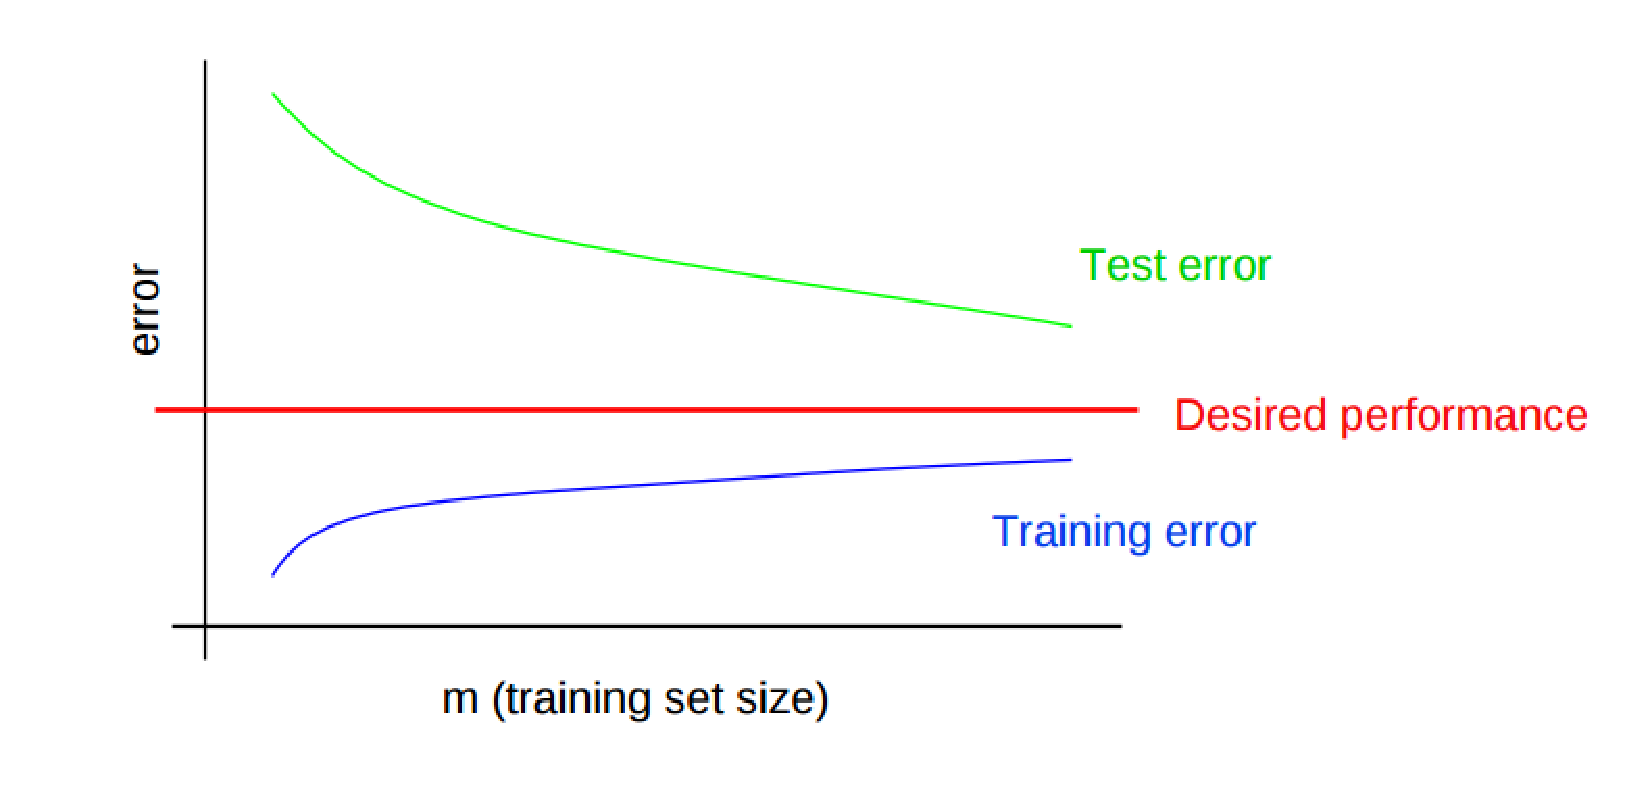
\includegraphics[width=0.9\textwidth]{figuras/curva_aprendizado.eps}
  \caption{Exemplo de uma curva de aprendizado \cite{1_ng} }
  \label{fig:curva_aprendizado}
\end{figure}

Pode-se ver na figura \ref{fig:curva_aprendizado}, o eixo das ordenadas representa
o valor do erro, enquanto o eixo das abscissas representa o tamanho do conjunto de
dado usado para treinamento. Para calcular o erro apresentado nos gráficos, pode-se
usar qualquer fórmula estatística para tal fim. Entretanto, uma das mais comuns
quando se trata de validação cruzada é a seguinte \cite{1_ng}:

\begin{equation}
ErroTreinamento = \frac{1}{2m}*\sum_{i=0}^{m}(h(x_{i}) - y(x_{i}))^2
\end{equation}

\begin{equation}
ErroTeste = \frac{1}{2m_{teste}}*\sum_{i=0}^{m_{teste}}(h(x_{t}^{i}) - y(x_{t}^{i}))^2
\end{equation}

Onde:

\begin{itemize}
    \item \textbf{m: } Tamanho do conjunto de teste;
    \item \textbf{$h(x_{i}$): } Função que reflete o modelo criado por um algoritmo
    de aprendizado de máquina, ou seja, recebe um dado e retorna um classificação.
    \item \textbf{$y(x): $} Valor real da classificação para o dado sendo apresentado
    \item \textbf{$m_{teste}$: } Tamanho do conjunto de teste obtido por validação cruzada.
\end{itemize}

Dessa forma, pode-se ver que o gráfico mostra a evolução do modelo produzido pelos
dados de treinamento em relação ao conjunto de dados obtidos pela validação cruzada,
variando-se o número de dados usados no treinamento. Espera-se que, inicialmente, as
curvas fiquem bem distantes uma da outra, pois com poucos dados de treinamento, o
conjunto de teste apresentará erros altos, enquanto o conjunto de treinamento
não sofre do mesmo problema. Entrentanto, com mais dados de treinamento usados,
é esperado que as curvas se aproximem mais uma da outra.

O uso desses gráficos pode-se bastante útil para encontrar casos de \textit{overfitting}
e \textit{underfitting} pois tais casos podem ser claramente identificados observando-se
o gráfico. Em um conjunto de teste onde ao final, as curvas de treinamento e de erro estão
muito distantes, pode-se entender que o algoritmo está apresentando \textit{underfitting}.
Entretanto, caso as curvas estejam muito próximas quando se usa todos os dados de
treinamento alocados, pode-se entender uma baixa variância do modelo, identificando assim
um caso de \textit{overfitting}.
